%!TEX root = ../thesis.tex

\chapter{Grundlagen}

In diesem Kapitel werden die mathematischen Grundlagen erläutert und die wesentlichen Konzepte hinter dem behandelten Verschlüsselungs-Algorithmus beschrieben. \\

%%%%%%%%%%%%%%%%%%%%%%%%%%%%%%%%%%%%%%%%%%%%%%%%%%%%%%%%%%%%%
\section{Gruppen und Endliche Körper}

Eine abelsche Gruppe im mathematischen Sinn ist ein Tupel $(G,\circ)$ aus einer nicht-leeren Menge G und einer darauf definierten inneren Verknüpfung $\circ$ (vgl. \cite{puttmann}, S. 11f). Hierbei entspricht die innere Verknüpfung einer Abbildung 
\begin{center}
$ \circ: X \times X \to X $
\end{center}
die jedem Paar $(x_1,x_2)$ aus Elementen der Menge X ein Element $x_1 \circ x_2$ zuordnet. Außerdem sind folgende Bedingungen auf der Struktur einer Gruppe definiert: \\

\begin{enumerate}
  \item Menge $G$ ist abgeschlossen, d.h. für alle $a,b \in G$ gilt, d.h. dass auch jede Verknüpfung $a \circ b$ ein Element von $G$ ist. 
  \item Assoziativgesetz: $ \forall a,b,c \in G: (a \circ b) \circ c = a \circ (b \circ c) $
  \item Kommutativgesetz: $ \forall a,b \in G: a \circ b = b \circ a $
  \item Neutrales Element: $ \forall a \in G: a \circ e = e \circ a = a$
  \item Inverses Element: $ \forall a \in G: a \circ a^{-1} = a^{-1} \circ a = e$\\
\end{enumerate}

Ein Beispiel für eine so definierte abelsche Gruppe entspricht der Menge der ganzen Zahlen $\mathbb{Z}$ mit der Addition als Verknüpfung $(\mathbb{Z},+)$. Die Anzahl der Elemente einer Gruppe wird als Ordnung bezeichnet, welche für die ganzen Zahlen unendlich ist. In der Kryptographie kommen jedoch stets Gruppen mit einer endlichen Anzahl von Elementen zum Einsatz, bei denen also die Ordnung der Gruppe beschränkt ist. \\

Eine besondere Form endlicher Gruppen bilden zyklische Gruppen, die ein Element $g$ besitzen, aus dem durch Verknüpfungen $\circ$ alle anderen Elemente der Gruppe erzeugt werden können. Das Element $g$ ist das sog. Generatorelement der zyklischen Gruppe $(G',\circ)$. \\ 

Eine Körper ist eine Erweiterung von abelschen Gruppen und als Tripel $(K,+,\cdot)$ definiert, welche zu einer nicht-leeren Menge $K$ konkret die inneren Verknüpfungen Addition und Multiplikation beschreibt. Folgende Bedingungen werden dabei erfüllt (vgl. \cite{pullmann}):

\begin{enumerate}
  \item Die Menge $K$ bildet durch die additive Verknüpfung $+$ eine abelsche Gruppe
mit 0 als neutralem Element
  \item Die Menge $K\setminus\{0\}$, d. h. $K$ ohne das Element 0, bildet durch die multiplikative Verknüpfung $\cdot$ ebenfalls eine abelsche Gruppe mit 1 als neutralem Element
  \item Distributivgesetz: $ \forall a,b,c \in K: c \cdot (a + b) = c \cdot a + c \cdot b $
\end{enumerate}

Unter einem Endlichen Körper\footnote{auch: Galoiskörper, finites Feld} versteht man einen Körper mit endlich vielen Elementen, der oft auch als Restklassenkörper bezeichnet wird. Ein Beispiel dafür sind Primkörper mit Primzahl $p$ und den Verknüpfungen \textit{Addition modulo p} und \textit{Multiplikation modulo p}: $\mathbb{Z}_p = \{0,1,2,3,\cdots,p-1\}$. \\

Galoiskörper werden mit $GF(p)$ abgekürzt, wobei $q$ eine Primzahl sein muss und für die Anzahl der Elemente im Feld steht. $GF(p)$ repräsentiert damit einen Körper der Restklasse ganzer Zahlen modulo $p$. Durch die mathematischen Eigenschaften dieser Struktur um Restklassen und inverse Elemente eignen sie sich besonders für den Einsatz in der Kryptographie. \\


%%%%%%%%%%%%%%%%%%%%%%%%%%%%%%%%%%%%%%%%%%%%%%%%%%%%%%%%%%%%%
\section{Elliptische Kurven}

Eine elliptische Kurve $E$ über ein finites Feld $F_p$ wird mit Hilfe der Weierstraß-Gleichung definiert:

% E:y2+a1xy+a3 y=x3+a2x2+a4x+a6
\begin{center}
$E: y^2 + a_1 x y + a_3 y = x^3 + a_2 x^2 + a_4 x + a_6 $
\end{center}

Die Parameter $a_1 \dots a_6$ legen fest, welche Form die elliptische Kurve annimmt und sind Elemente des finiten Feldes $F_p$. Sie werden durch die Domain-Parameter festgelegt. 

\begin{figure}[H]
	\centering
   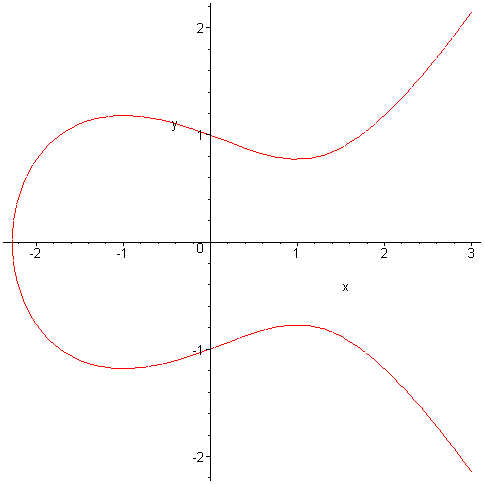
\includegraphics[width=0.60\textwidth]{bilder/ellkurve}
	\caption{Graph einer Elliptischen Kurve}
	\label{ellkurve}
\end{figure}

Über eine Reihe von Vereinfachungen lässt sich die Weierstraß-Gleichung auf die folgende Formel reduzieren:  % y2 mod p=x3+ax+b mod p 
\begin{center}
$ y^2 \bmod p = x^3 + a x + b \bmod p $
\end{center}


Damit eine elliptische Formel in der Kryptographie eingesetzt werden kann, muss zusätzlich folgende Bedingung gelten: %4a3+ 27b2 mod p 0
\begin{center}
$ 4 a^3 + 27 b^2 \bmod p \ne 0 $
\end{center}

Das neutrale Element der Gruppe wird mit O gekennzeichnet und beschreibt einen Punkt im Unendlichen. \\


%%%%%%%%%%%%%%%%%%%%%%%%%%%%%%%%%%%%%%%%%%%%%%%%%%%%%%%%%%%%%
\section{Das diskrete Logarithmus-Problem}


%%%%%%%%%%%%%%%%%%%%%%%%%%%%%%%%%%%%%%%%%%%%%%%%%%%%%%%%%%%%%
\section{Digitale Signaturen}


%%%%%%%%%%%%%%%%%%%%%%%%%%%%%%%%%%%%%%%%%%%%%%%%%%%%%%%%%%%%%
\section{ECDSA-Algorithmus}

\subsection{Signatur}

\subsection{Verifikation}

